\chapter{Design}
\frame{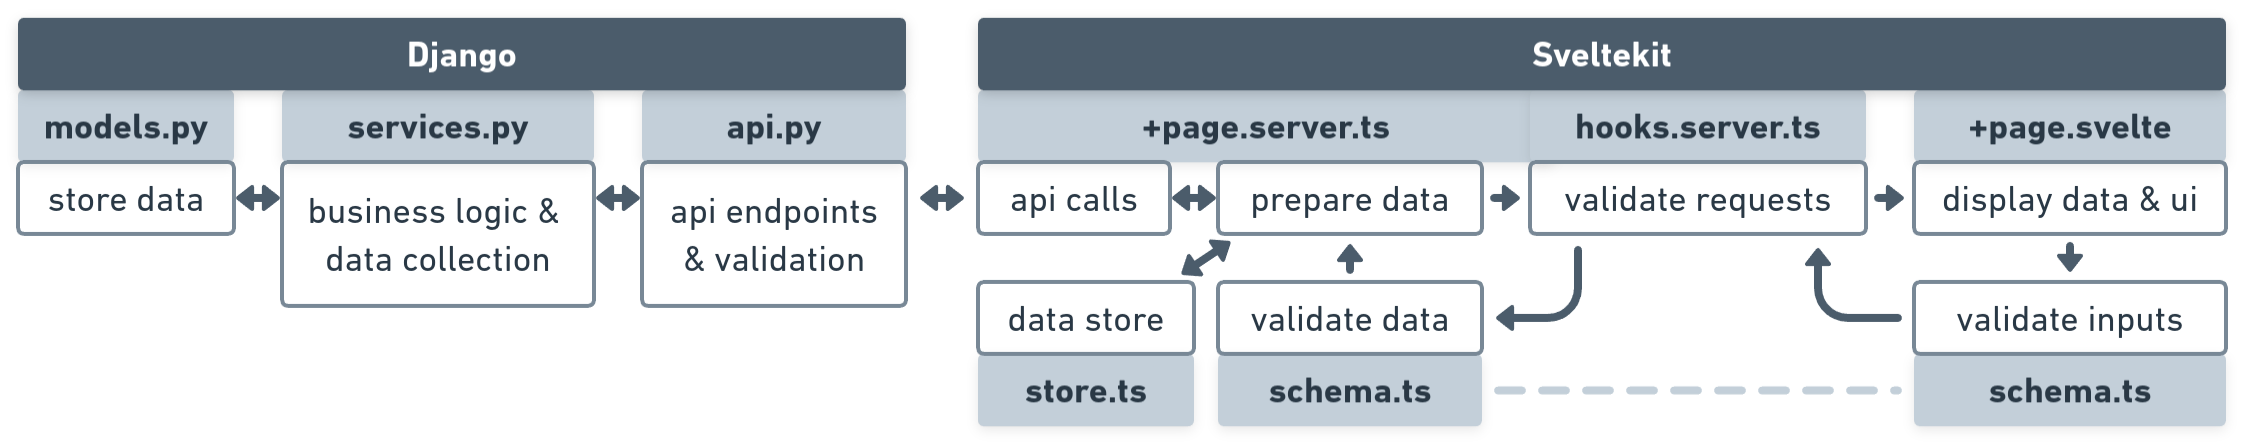
\includegraphics[width=\linewidth]{images/design.png}}
The following paragraphs will be edited to explain their advantages specifically for this project - rather than just being a general description.

Good design follows C.R.A.P principles. It is Consistent, it is Readable, it is Accessible, and it is Predictable. (SOURCE) This is a idea by a german ... for example in our design...

We can also take ideas from Normans and the three paradigms of HCI (source source)

The choice of background color in this project (dark and gray and light more) (source). The dotted background in lightmode gives users a .... easier on the eyes ... dark mode for those working late (which is common) ...

This project uses the Noord font (source), a relatively unknown but very modern and clean... sans-serif because ...

Shadcn-Svelte, a library for SvelteKit (see 3.2), created by Huntabyte, makes designing the User Interface easy. It also depends on a collection of Svelte-based tools and libraries aimed at enhancing web development workflows. This includes zod, and formsnap (which relies on superforms), which allows validation to be done on the client side. This allows for a responsive user experience which...

Shadows give a ...

The purple color is chosen because the RCR... Red for the logout button (source)
\section{Backend}
Django is a high-level Python web framework that enables rapid development of secure and maintainable websites. It takes care of much of the hassle of web development, so you can focus on writing your app without needing to reinvent the wheel. It follows the "battery-included" philosophy and provides a robust set of features to build web applications. It emphasises reusability and "pluggability" of components, less code, low coupling, rapid development, and the principle of don't repeat yourself (DRY). (SOURCE)

It is preferred over XYZ because…

Django-Ninja is a web framework for building APIs with Django and Pydantic. It is designed to be fast, easy to use, and type-safe. Django-Ninja leverages the Pydantic library for data validation and settings management using Python type annotations. This integration ensures that API requests and responses are type-checked, leading to cleaner and more maintainable code. It aims to provide a more intuitive and productive way to build Django APIs, with automatic OpenAPI documentation generation and much faster performance. (SOURCE)

It is preferred over Django Rest Framework because….

Django-Ninja-JWT is an extension for Django-Ninja, through Django-Ninja-Extra, that provides JSON Web Token (JWT) authentication for APIs. It allows for secure and scalable user authentication using JWTs. This tool integrates seamlessly with the Django-Ninja framework, enabling developers to easily add token-based authentication to their API endpoints. (SOURCE) It will be stored in a http only, same site strict cookie to ensure security. 

CSRF token handling within django is not required, as the Django backend will not be connected to the internet at all, and SvelteKit handles anti CSRF protection by default. (SOURCE)

\section{Frontend}
SvelteKit is a framework for building web applications using Svelte, a modern JavaScript compiler that produces highly efficient code. SvelteKit provides a seamless development experience by offering server-side rendering, static site generation, and single-page application modes out of the box. It is designed to be flexible and modular, allowing developers to structure their applications as they see fit, while providing a rich set of tools and features to enhance productivity and performance. (Source)

It is preferred over React and Vue3 because…

TypeScript is an open-source programming language developed and maintained by Microsoft. It is a strict syntactical superset of JavaScript, adding optional static typing to the language. TypeScript is designed for the development of large applications and trans compiles to JavaScript. It can catch errors and bugs at compile time, providing a more robust and maintainable codebase. (Source)


Axios is a promise-based javascript library, which provides a more streamlined and readable syntax than Fetch for handling asynchronous operations. It will be used by django to perform CRUD operations. It features a wide array of configurations and supports features such as intercepting requests and responses, cancelling requests, and automatic transformation of request and response data. (Source)

openAPI-typescript allows us to import the django-ninja openAPI schema into the frontend, providing type safety and autocompletion. This ensures that the frontend and backend are always in sync, reducing the likelihood of errors and inconsistencies. (Source)

Postmark is an email delivery service that provides fast and reliable transactional email sending. Its simple yet robust API will allow easy email verification and notifications directly from SvelteKit. It is preferred over self-hosted emailing as those are usually blocked as spam by all major email services. (source)

\section{Deployment}
The project is depoloyed on an ubuntu server with nginx, gunicorn, and node (Elaborate on the reasons) sveltekit has adaptors to ... (sources)

\section{Requirements}
This is the state machine diagram for the system to use for JDs. It is used in the UI to show the user what stage the JD is at, and updates automatically on button press when an update is made.

\noindent
\frame{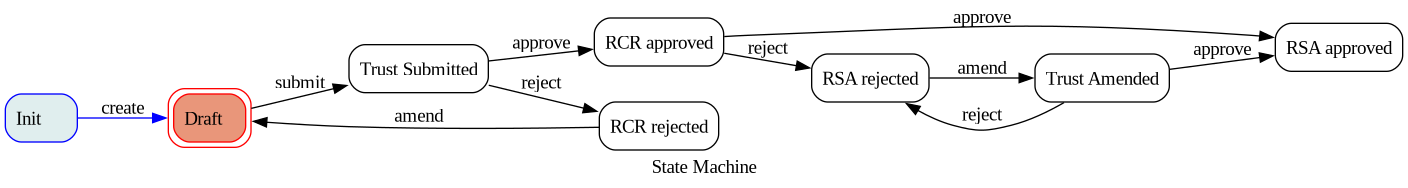
\includegraphics[width=\linewidth]{images/jd-state-machine.png}}

\noindent
\frame{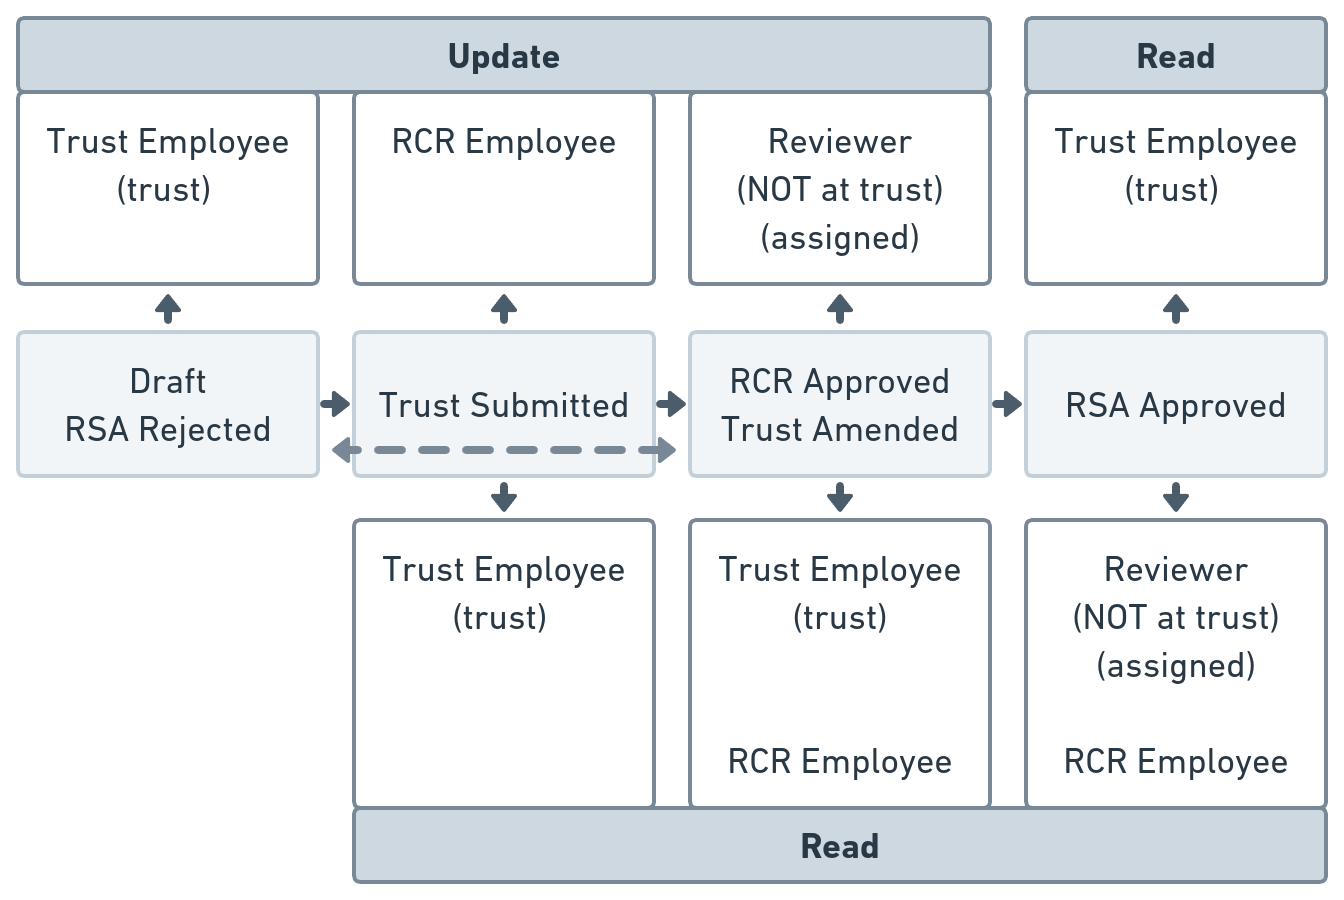
\includegraphics[width=0.5\linewidth]{images/perms.png}}